\chapter{{\color{done}Упрощения уравнений гидротермодинамики}}
    \begin{warn}
    Сюда нужен вводный текст. Сказать про не решаемость уравнений НС и про необходимость выкручиваться. 
    \end{warn}

\section{{\color{done}Упрощения уравнений на основе масштабного анализа и физических аргументов}}

Система (\ref{mom_conserv_turb_u})-(\ref{temp_conserv_turb}), хотя в ней и было проведено "сглаживание" в основном для того, чтобы заменить молекулярную вязкость и теплопроводность на их турбулентные аналоги, отражает движения многий масштабов, начиная от быстрый акустических и гравитационных колебаний и заканчивая медленными волнами синоптического или планетарного масштаба. Поэтому исходная система (\ref{mom_conserv_turb_u})-(\ref{temp_conserv_turb}) как правило упрощается, исходя из того, какие процессы в атмосфере мы хотим изучать, а воспроизведением каких движением мы можем, или даже лучше пожертвовать, чтобы не вносить дополнительный шум. Те или иные упрощения в исходной системе производятся как правило исходя из некоторых общих физических соображений и последующего масштабного анализа или путем оценки порядка величин отдельных членов уравнений, исходя из известных характерных значений переменных, их вертикальных и горизонтальных производных.

Например, при изучении крупномасштабной динамики в свободной атмосфере сразу делается предположение, что силы трения вдали то земной поверхности невелики и уже затем производится дальнейший масштабный анализ для уравнений невязкой жидкости. Напротив, в пограничном слое сразу делается предположение, что силы трения важны, а горизонтальная изменчивость переменных несущественна и производится отбрасывание соответствующих членов.

Следует отметить, что масштабирование применительно к атмосфере проводить не совсем просто, ибо атмосфера Земли, как уже отмечалось ранее, имеет довольно большое отношение аспекта $A=L/h$. Отношением аспекта называют также отношение горизонтального размера той или иной циркуляционной ячейки к ее вертикальному размеру. Например, горизонтальный размер (масштаб) циклона или антициклона $L=10^3$км, а его вертикальная мощность $h = 10$км, то есть $A_{циклона}  \simeq 10^2$. Кучево-дождевые облака имеют примерно одинаковый размер по вертикали и горизонтали, т.е. для него $A \simeq 1$. Этот факт также нужно учитывать при масштабировании и оценке различных членов в уравнениях. В качестве исходных масштабов всегда лучше брать основные: масса $(\tilde{M})$, время $(\tilde{t})$, длина $(L)$. Так как отношение аспекта для атмосферы много больше единицы, то масштаб масштаб длины может быть различным по горизонтали и вертикали и тогда, строго говоря, нужно переходить к вертикальному масштабированию. Однако сейчас мы остановимся на в рамках традиционного для метеорологии квазискалярного масштабирования, подразумевая под масштабом $L$ горизонтальный масштаб возмущений. С определением горизонтального масштаба проблем как правило не возникает, поскольку из опыта мы хорошо знаем горизонтальные масштабы (размеры) различных атмосферных возмущений: циклонов, планетарных волн , конвективных образований. Интерпретация масштаба времени не столь однозначна. Что подразумевать под масштабом времени? Имеются различные возможности. Под масштабом времени можно  подразумевать характерное время жизни того или иного атмосферного образования. Например, характерное время жизни циклона составляет 4-5 дней. Если примем характерное время жизни 4 дня, то это составит $3600\times24\times4\simeq3.6\times10^5$с. 

Наиболее часто масштабом времени является так называемся адвективный масштаб, который определяется через линейный масштаб атмосферного образования и скорость ветра в нем. Недостаточно такого подхода является то, что время выступает в этом случае вторичным масштабом $\tilde{t}=\frac{L}{\tilde{U}}$. В случае простой циркуляции такой масштаб является по существе характерный временем оборота частицы в той или иной системе циркуляции. Например, если возьмем частицу, находящуюся на расстоянии 100 км от центра циклона и положим, что скорость ветра составляет 20 м/с то характерный масштаб времени $\tilde{t}=\frac{10^6m}{20 m/s}=5\cdot 10^4s$. То есть определенный таким образом масштаб времени становится на порядок меньше, чем масштаб, определенный по характерному времени жизни циклонического возмущения. Здесь же можно добавить, что адвективные масштабы времени частиц, находящихся на разных расстояниях от циклона будут весьма отличными. Между тем масштаб времени указывает на то, сколь существенно для той или иной циркуляции учитывать силы Кориолиса. Если характерный масштаб времени $\geq$ суткам $=\Omega^{-1}$, то влияние силы Кориолиса существенно, если заметно меньше, что несущественно. Если мы берем адвективный масштаб времени, то требуем, чтобы характерное время обращения частицы в данной циркуляции составляло сутки или более . На самом деле частица можно совершать несколько оборотов и течение жизни циклона, т.е. реальное время воздействия на нее силы Кориолиса будет заметно больше адвективного масштаба времени. Естественно, что адвективный масштаб времени всегда меньше времени жизни системы, поэтому можно ожидать, что при таком выборе масштаба времени влияние силы Кориолиса на более мелкомасштабные, но долгоживущие системы типа тропических циклонов, бризов может недооцениваться. Если мы останемся в рамках адвективного масштаба времени, то возможность учета вращения будет определяться условием 
\begin{equation}
    \frac{L}{\Tilde{U}}\geq \left( 2\Omega \right)^{-1}
\end{equation}
или, что эквивалентно, 
\begin{equation}
    \varepsilon=\frac{\Tilde{U}}{2\Omega L}\leq 1,
\end{equation}
где $\varepsilon$ -- безразмерный параметр, называемый числом Россби. Ради справедливости следует отметить, что впервые этот параметр встречается в работе {\color{warn} Кибеля 1940 г}, поэтому правильнее его было бы называть числом Кибеля. Так, в соответствии с таким масштабированием к крупномасштабным явлениям относят процессы, угловая скорость которой $\left( \frac{\Tilde{U}}{L} \right)$ меньше угловой скорости Земли. Число Россби можно интерпретировать как отношение этих угловых скоростей.

Обратимся теперь к нашим уравнениям движения, переписав их в несколько ином виде, объединив все члены в правой части, кроме ускорения Кориолиса, в один член. Тогда уравнения движения в векторной форме примут вид
\[
    \td{\vec{U}}{t}+2\Omega\times\vec{U}=\vec{F}
\]
Относительное ускорения имеет порядок 
\begin{equation}
\label{eq:ch4-1}
    \td{\vec{U}}{t}=O\frac{\Tilde{U}}{L},
\end{equation}
т.к. мы приняли выше, что $\Tilde{t}=\frac{L}{\Tilde{U}}$, а ускорение Кориолиса имеет порядок
\begin{equation}
    \label{eq:ch4-2}
    2\Omega\times\vec{U}=O\left(2 \Omega \Tilde{U}\right)
\end{equation}
Разделив (\ref{eq:ch4-1}) на (\ref{eq:ch4-2}), будем иметь
\begin{equation}
    \label{eq:ch4-Rossby}
    \varepsilon=\frac{\Tilde{U}}{2\Omega L},
\end{equation}
т.е. число Россби. Условие $\varepsilon<1$ обозначает, что относительное ускорение играет в этом случай значительно меньшую роль, чем ускорение Кориолиса. т.е. воздействие сил $\vec{F}$ балансируется в основном силой Кориолиса. Единственное но, которое может возникнуть при интерпретации (\ref{eq:ch4-Rossby}) состоит в том, что из этого выражения следует, что чем больше масштаб движения, тем больше преобладает ускорение Кориолиса над относительным ускорением.

Поясню это "но". Если бы мы взяли в качестве исходных масштабов $L$-длины, $\Tilde{t}$-времени, то имели бы $\Tilde{U}=\frac{L}{\Tilde{t}}$.  Тогда
\[
\td{\vec{U}}{t}=O\left(\frac{L}{\Tilde{t}^2}\right), \:\: 2\Omega\times\vec{U}=O\left( 2\Omega\frac{L}{\Tilde{t}}\right)
\]
Аналогом числа Россби стало бы выражение 
\[
\varepsilon_1=\frac{\cancel{L} \cancel{\Tilde{t}}}{\Tilde{t}^{\cancel{2}} 2 \Omega \cancel{L} }=\frac{1}{\Tilde{t} 2 \Omega}=\frac{1}{\Tilde{t}\cdot 10^{-4}}
\]
т.е. при $\Tilde{t}\geq 10^4\simeq3$ч, а $\varepsilon<1$, т.е. интерпретация была бы таковой. Для любых движения с масштабом времени более 3ч ускорение Кориолиса преобладает над относительный ускорением. Как видите, линейный масштаб оказывается здесь отсутствующим. Это более правильная формулировка. На практике действительно системы большего линейного масштаба имеют и большее характерное время жизни, поэтому больших противоречий между двумя определениями числа Россби нет. 

Итак, в случае идеальной жидкости из приведенного анализа следует выполнение условия квазигеострофичности, т.е.
\[
2\vec{\Omega}\times\vec{U}\simeq -\frac{1}{\rho}\nabla p - \vec{g}
\]
Так как ускорение силы тяжести присутствует только в третьем уравнении движения, сравним это ускорение с относительным ускорением
\[
\td{w}{t}+\vec{g}=\vec{F},
\]
где $\vec{F}$ - все остальные действующие силы. Используя масштаб времени $\Tilde{t}$ и вертикальный масштаб $L_z$ получим
\[
\td{w}{t}=O\left(\frac{L_z}{\Tilde{t}^2g}\right)
\]
и отношение
\begin{equation}
    \label{eq:ch4-Gscale}
    G=\frac{L_z}{\Tilde{t}^2g},
\end{equation}
характеризующее важность относительных ускорений по сравнению с ускорением силы тяжести. Условие $G<1$ свидетельствует о мало вкладе относительных ускорений. Т.к. $z$ для большинства циркуляций ограничен толщиной тропосферы, то примем $L_z=10^4$м. Тогда будем иметь $G \simeq \frac{10^3}{\Tilde{t}^2}<1$ выполняющееся для большинства метеорологически значимых циркуляций. Только для циркуляций с характерным временем порядка 30 с во всей толще тропосферы относительное ускорение имеет тот же порядок, что и сила тяжести. С ростом характерного времени жизни (масштаба времени) возмущений стремление к гидростатичности увеличивается. Потому при рассмотрении крупномасштабных атмосферных движений относительное ускорение игнорируется и прогностическое уравнение заменяется уравнением гидростатики. При теоретическом и численном изучении сравнительно быстрых процессов (конвекции, гравитационных волн) продолжительность которых составляет $O[10^3-10^4]$c относительные ускорения учитываются, хотя из соотношения (\ref{eq:ch4-Gscale}) видно, что даже в этом случае $G\ll1$.

Некоторые дополнительные упрощения исходных уравнений проводятся на основании оценки порядка различных членов в уравнениях, исходя из характерных значений как самих функций, так и их производных. В книге П.Н.Белова "Численные методы прогноза погоды", Л.Гидрометиздат, 1975 на стр 13 имеется таблица таких значений для крупномасштабных движений. Исходя из этих значений их рассмотрения удаляется член $l_1w$ в уравнении движения для компонента $u$, а такие же вязкие члены, аналогично из уравнения для $v$ -- вязкие члены, из уравнения для $w$ само ускорение, члены с ускорением Кориолиса и вязкие члены, т.е. уравнение сводится к уравнению гидростатики. В уравнении притока тепла исключаются члены с теплопроводностью. 

Завершая этот раздел отметим, что сохранение или исключение из полных уравнений тех или иных членов очень сильно зависит от характера решаемой задачи, поэтому формулировка математической модели выбирается исходя из характерных свойств изучаемого процесса. 

\section{{\color{done}Некоторые стационарные формы течений}}

\subsection{{\color{done}Состояние покоя}}
    В состояний покоя уравнения движения (\ref{mom_conserv_turb_u}, \ref{mom_conserv_turb_v} и \ref{mom_conserv_turb_w}) свелось бы к уравнению гидростатики
    \begin{equation}
    \label{hydrostatic}
        \pd{p}{z} = -\rho g
    \end{equation}
    и мы имели бы дополнительно $\pd{p}{x}=0$, $\pd{p}{y}=0$ или 
    \begin{equation}
    \nabla_h p=0    
    \end{equation}
    Уравнение неразрывности (\ref{mass_conserv_turb}) приобрело бы вид 
    \begin{equation}
    \label{no_hor_pressure}
        \pd{\rho}{t} = 0
    \end{equation}
    Мы можем применить соотношение (\ref{no_hor_pressure}) к уравнению (\ref{hydrostatic}) и получим
    \begin{equation}
    % \label{no_hor_pressure}
        \frac{\partial}{\partial z}\nabla_h p = -g \nabla_h p = 0,
    \end{equation}
    так что горизонтальные градиенты плотности исчезают. Раз исчезают горизонтальные градиенты плотности и горизонтальные градиенты давления , то из уравнения состояния
    \begin{equation}
    \label{state_eq}
        p = \rho R T
    \end{equation}
    следует, что горизонтальные градиенты температуры также должны исчезнуть. Таким образом мы показали, что если скорости и ускорения исчезли, то должны исчезнуть и горизонтальные градиенты температуры. Верно и обратное: пока имеются горизонтальные градиенты температуры, будут существовать движения и ускорения.

    Рассмотрим наконец уравнение притока тепла (\ref{temp_conserv_turb}) при отсутствии скоростей, ускорений и горизонтального градиента давления. В этом случае оно приобретает вид
   \begin{equation}
    \label{dtheta_dt}
        \pd{\theta}{t} = \frac{\theta}{T}\frac{1}{\rho c_p}\left( -\pd{F}{z} \right)+\frac{\partial}{\partial z}\kappa\pd{\theta}{z} 
    \end{equation}
    Покажем, что в состоянии покоя должны исчезнуть и  локальные изменения температуры. Из уравнения (\ref{no_hor_pressure}) имеет, что $\rho$ стационарно, поэтому, продифференцировав (\ref{hydrostatic}) по времени имеем
    \begin{equation}
    \label{dtd_dpdz}
        \pd{}{t}\left(\pd{p}{z}\right) = \frac{\partial}{\partial t}(-\rho g)=0, \:\: \Rightarrow   \:\:  \pd{p}{t}=0
    \end{equation}
    Из уравнения состояния (\ref{state_eq}) при условиях (\ref{no_hor_pressure}) и (\ref{dtd_dpdz}) имеем
    \begin{equation}
    % \label{dtd_dpdz}
        \pd{T}{t} = 0.
    \end{equation}
    Если $\pd{T}{t} = 0$, $\pd{p}{t} = 0$, то $\pd{\theta}{t} = 0$ и имеем (\ref{dtheta_dt}) в виде
   \begin{equation}
    % \label{dtheta_dt}
        \frac{\theta}{T}\frac{1}{\rho c_p}\left( -\pd{F}{z} \right)=\frac{\partial}{\partial z}\kappa\pd{\theta}{z}, 
    \end{equation}
    то есть вертикальный профиль определяется дивергенцией радиационных процессов. Если радиационный приток тепла  отсутствует, то $\kappa\pd{\theta}{z}=const$, а при $\kappa=const$ 
\begin{warn}
Сказать, что $\kappa=const$ -- это наиболее распространенный способ задания коэффициента теплопроводности. Ньютоновская жидкость?  
\end{warn}
   \begin{equation}
        \theta = Az+C. 
    \end{equation} 
    То есть в состоянии покоя вертикальный профиль температуры может быть только линейным.


\subsection{{\color{done}Геострофический поток}}
    Если введем теперь упрощения, упомянутые в конце раздела 4.1 (идеальная жидкость, $f_h w = 0$, $\td{w}{t}=0$ и $f_h u = 0$), то система (\ref{mom_conserv_turb_u})-(\ref{temp_conserv_turb}) приобретает следующий вид:
    \begin{equation}
    \label{eq:DuDt_geost}
        \td{u}{t} = -\frac{1}{\rho}\pd{p}{x}+fv 
    \end{equation} 
    \begin{equation}
    \label{eq:DvDt_geost}
        \td{v}{t} = -\frac{1}{\rho}\pd{p}{y}-fu 
    \end{equation} 
    \begin{equation}
        0 = -\frac{1}{\rho}\pd{p}{z}-g 
    \end{equation} 
    \begin{equation}
        \pd{\rho}{t} + \pd{(\rho u)}{x} + \pd{(\rho v)}{y} + \pd{(\rho w)}{z} = 0 
    \end{equation} 
    \begin{equation}
    \label{eq:DthetaDt}
        \td{\theta}{t} = \frac{\theta}{T} \frac{1}{\rho c_p} + \varepsilon
    \end{equation} 
    Здесь для простоты $\varepsilon$  обозначает все притоки тепла. Дальнейшим упрощением является гидростатичность:
    \begin{equation}
        0 = -\frac{1}{\rho}\pd{p}{x}+fv, \:\: 0 = -\frac{1}{\rho}\pd{p}{y}-fu,  
    \end{equation} 
    откуда получаются значения компонентов геострофического ветра 
    \begin{equation}
        u_g = -\frac{1}{f \rho}\pd{p}{y}, \:\: v_g = \frac{1}{f \rho}\pd{p}{x},  
    \end{equation} 
    \begin{info}
    Не следует забывать, что геострофический ветер является гипотетическим движением, параллельным  изобарам. Эффекты трения и кривизны действительного потока, которые приводят центробежному ускорению частиц, в нем отсутствуют.
    \end{info}

    В случае несжимаемой жидкости ($\rho=const$) уравнение неразрывности принимает вид
    \begin{equation}
        \pd{u}{x}+\pd{v}{y}+\pd{w}{z}=0.  
    \end{equation} 

\subsection{{\color{done}Поток Куэтта}}
    Геострофический ветер является одним из типов стационарных решений, имеющих место в идеальной жидкости. Если жидкость вязкая, а характерное время не велико, то можно пренебречь влиянием силы Кориолиса. Если предположить дополнительно, что процесс стационарный, движение горизонтальное и однородное, а жидкость несжимаема, то уравнения Навье-Стокса, обсуждавшиеся ранее, или уравнения осредненных движений с $\nu=const$? приобретут следующий вид
    \begin{equation}
        -\frac{1}{\rho}\nabla_h p + \nu\frac{\partial^2 \vec{V}}{\partial z^2}=0.  
    \end{equation} 
    Здесь $\nabla_h=\frac{\partial}{\partial x }+\frac{\partial}{\partial y }+\frac{\partial}{\partial z }$, $\:\:\vec{V}=\vec{i}u+\vec{j}v$.
    Если предположить дополнительно, что $\nabla_h p = 0$, то будем иметь
    \begin{equation}
        \frac{\partial^2 \vec{V}}{\partial z^2}=0.  
    \end{equation} 
    Решением этого уравнения будет 
    \begin{equation}
        \vec{V}=\vec{V_0}+\vec{\gamma}z; \:\: u=u_0+  \gamma z; \:\: v=v_0+  \gamma z.
    \end{equation} 
    Такого рода поток с линейным профилем скорости называют обычно потоком Куэтта (Рис. \ref{fig:simple_flows}). Он очень удобен при задании фонового потока в задачах мезометеорологии.

\subsection{{\color{done}Поток Пуазейля}}
    
    Если мы примем теперь, что горизонтальный градиент давления постоянен  $\frac{1}{\rho}\nabla_h p=\vec{G}$, то будем иметь
    \begin{equation}
        \nu\frac{\partial^2 \vec{V}}{\partial z^2}=\vec{G} 
    \end{equation} 
    \begin{equation}
        \frac{\partial^2 \vec{V}}{\partial z^2}=\frac{\vec{G}}{\nu}  
    \end{equation} 
    \begin{equation}
        \pd{\vec{V}}{z}=\frac{\vec{G}}{\nu}z+\vec{a}.  
    \end{equation} 
    \begin{equation}
        \vec{V}=\frac{\vec{G}}{\nu}z^2+\vec{a}z+\vec{V_0}. 
    \end{equation} 
    То есть профиль ветра становится параболическим и для составляющих скорости принимает вид
    \begin{equation}
    \begin{aligned} 
        u &= \frac{1}{\nu\rho} \pd{p}{x}z^2 + az + u_0 \\
        v &= \frac{1}{\nu\rho} \pd{p}{y}z^2 + az + v_0 
    \end{aligned} 
    \end{equation} 
    Этот поток называется потоком Пуазейля, его также удобно использовать в качестве фонового потока в мезометеорологии и пограничного слоя. Вообще нужно отметить, что уравнения движения позволяют получить весьма ограниченное количество аналитических стационарных решений. Кроме геострофического потока, потока Куэтта и Пуазейля позже будет рассмотрен поток Экмана, в котором помимо силы вязкости учитывается также сила Кориолиса. Это будет сделано при изучении особенности атмосферных движений в пограничном слое атмосферы. 

    \begin{figure}[!h]
    \label{fig:simple_flows}
    \caption{Вертикальные профили скорости при потоках Куэтта и Пуазейля}
    \centering
    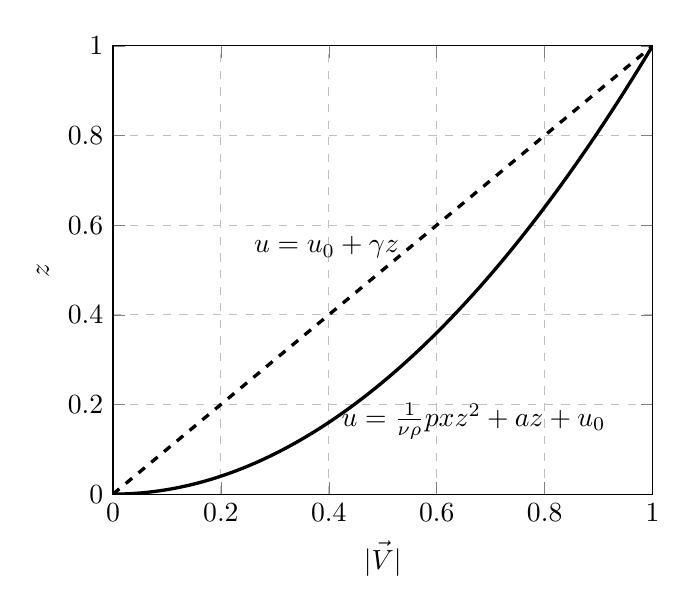
\begin{tikzpicture}
    \begin{axis}[xmin=0,ymin=0,xmax=1,ymax=1,
    xlabel=$\vec{|V|}$, 
    ylabel=$z$, 
    % title={title титуль},
    xmajorgrids=true,
    ymajorgrids=true,
    grid style = dashed]
    \addplot[domain=0:1,color=black, dashed, very thick, samples=8]{x}node[left,pos=0.55]{$u=u_0+  \gamma z$};
    \addplot[domain=0:1,color=black, very thick, samples=200]{x^2} node[right,pos=0.3]{$u=\frac{1}{\nu\rho} \pd{p}{x}z^2 + az + u_0$};
    \end{axis}
    \end{tikzpicture}
    \end{figure}


\section{{\color{done}Уравнения движения на $\beta$-плоскости, $\beta$-эффект}}
    \begin{warn}
        Переписать на более понятный язык!
    \end{warn}
    Предыдущем разделе были выписаны упрощенные уравнения движения (\ref{eq:DuDt_geost}), (\ref{eq:DvDt_geost}) для идеальной жидкости. Повторим их заново, расписав в явном виде член с ускорением Кориолиса
    \begin{equation}
    \label{DuDt_geost_cor}
        \td{u}{t} = -\frac{1}{\rho}\pd{p}{x}+2\omega \sin\varphi v
    \end{equation} 
    \begin{equation}
    \label{DvDt_geost_cor}
        \td{v}{t} = -\frac{1}{\rho}\pd{p}{y}-2\omega \sin\varphi u
    \end{equation} 
    Здесь $\omega$ -- угловая скорость вращения Земли, $\varphi$ -- широта местности.  Как уже говорилось, в локальной декартовой предполагается, что плоскость $XOY$ касается поверхности Земли в точке $O$, совпадающей с началом координат, ось $у$ направляется на север вдоль меридиана, а ось $x$ на восток вдоль широты. В членах, описывающих силу Кориолиса, присутствует, однако, широта местности.
    
    Если размеры области невелики и зависимостью от силы Кориолиса можно пренебречь, т.е. принять $2\Omega \sin\phi_0=f_0=const$, где $\phi_0$ -- широта местности в точке $O$ декартовой системы координат. В этом случае говорят, что задача решается на $\beta$-плоскости.
    Часто бывает, однако, удобно не прибегая к сферической системе координат рассматривать ту или задачу динамики атмосферы в достаточно большой широтном поясе и учесть приближенно изменение силы Кориолиса с широтой. При этом желательно, чтобы для каждой точки в плоскости $XOY$ не приходилось рассматривать широту местности, присутствующую в исходных уравнениях. Система уравнений в локальной системе координат, где приближенно (линейно) учитывается изменение силы Кориолиса с широтой, называется системой уравнения на $\beta$-плоскости, где $\beta$ -- постоянный коэффициент, обеспечивающий учет линейного изменения силы Кориолиса с широтой. Ниже мы рассмотрим рассуждения, приводящие к системе уравнений на $\beta$-плоскости.
    Поскольку по начальному предположению мы хотим сохранить только линейную часть в измерении силы Кориолиса с широтой, естественно воспользоваться разложением функции в ряд Тейлора с сохранением только первого члена разложения. Обозначим $2\omega \sin\varphi =f$ и разложим $f$ в ряд Тейлора в точке, принятой за начало координат на широте $\phi_0$. Будем считать
    \begin{equation}
    \label{f_fourie}
        f = f_0 + \left. \pd{f}{y} \right|_{y=0} \cdot y, \:\: y=a\varphi,
    \end{equation} 
    где $a$ -- радиус Земли.
    \begin{equation}
    % \label{DvDt_geost}
        \left. \pd{f}{y} \right|_{y=0} = \left. \frac{1}{a}\frac{\partial}{\partial\varphi} \left( 2\omega \sin\varphi \right)\right|_{y=0} = \frac{2\omega}{a}\cos\varphi_0=\beta=const
    \end{equation}
    Поэтому константа $\beta=\frac{2\omega\cos\varphi_0}{a}$ дает скорость изменения силы Кориолиса с широтой и мы будем иметь  
    \begin{equation}
    \label{f_linear}
        f=f_0+\beta y    
    \end{equation}
    
    Оценим порядок $\beta$ на широте $\phi=60^o$: \\
    \[
        \beta=\frac{2 \cdot 7.26 \cdot 10^{-5}s{-1} \cdot 0.5}{6.38 \cdot 10^6 m} \simeq 10^{-11} m^{-1}s^{-1}
    \]
    Рассмотрим теперь, как это член соотносится по порядку величины с другими членами, например относительной завихренностью. Уравнение \ref{f_fourie} можно представить в следующем виде
    \begin{equation}
        \Delta f = \frac{1}{a}\pd{f}{\varphi}\Delta y.
    \end{equation}
    Далее, характерный масштаб относительного вихря $\zeta$ оценивается как
    \[ 
        \zeta = O \left[ \frac{U}{L} \right].
    \]
   Посмотрим теперь, при каких условиях $\Delta f$ будет порядка $\zeta$. Это будет при 
   \[
   2\omega\cos\varphi\frac{\Delta y}{a}=\frac{U}{L}
   \] 
   или 
   \[\cos\varphi\frac{\Delta y}{a} = \frac{U}{2\omega L}=\varepsilon,\] 
   где $\varepsilon$ -- число Россби.

   Если примем, что $O[\cos\varphi]=0.5$, то получим
   \[
   \Delta y = \frac{U \cdot a}{0.5 \cdot 2\omega L}.
   \]
   Приняв масштаб скорости $U=10$ м/с, масштаб длины $L=1000$ км, будем иметь
   \[
   \Delta y = \frac{10 m/s \cdot 6.3 \cdot 10^6 m \cdot 10^4 s}{1.5 \cdot 10^6 m \cdot 0.5} \simeq 4 \cdot 10^5 \simeq 800 km 
   \]
   
   Таким образом при характерных смещениях воздушных частиц в меридиональной плоскости $\geq800$ км изменение силы Кориолиса с широтой становится сравнимым по порядку с относительным вихрем и это изменение следует учитывать. Иными словами при масштабе рассматриваемых циркуляционных систем $\leq800$ км можно использовать систему уравнений на $f$-плоскости, при циркуляционных системах  $\geq800$ км учет сферичности Земли целесообразен и лучше пользоваться уравнениями на $\beta$-плоскости.
   
   Итак, модель, в которой геометрия движений предполагается плоской, несжимаемой, в параметр Кориолиса линейной функцией от $y$ (приближенный учет сферичности Земли), называется моделью на $\beta$-плоскости. С использованием (\ref{f_linear}) уравнения (\ref{DuDt_geost_cor}) и (\ref{DvDt_geost_cor}) примут следующий вид
    \begin{equation}
    % \label{DuDt_geost_cor}
        \td{u}{t} = -\frac{1}{\rho}\pd{p}{x}+f_0 v+\beta y v, 
    \end{equation} 
    \begin{equation}
    % \label{DvDt_geost_cor}
        \td{v}{t} = -\frac{1}{\rho}\pd{p}{y}-f_0 u+\beta y u. 
    \end{equation} 
    \begin{warn}
        В $p$-системе координат член с параметром Кориолиса при решении задачи на $\beta$-плоскости преобразуется точно так же, как и в рассмотренной выше $z$-системе координат, поскольку $y_z=y_p$ и используемые операторы $\frac{\partial}{\partial y}$ в обоих системах координат тождественны.\\
        ДОБАВИТЬ ЭТУ ФРАЗУ В УРАВНЕНИЯ В $P$-СИСТЕМЕ
    \end{warn}

\section{{\color{done}Уравнения мелкой воды}}
    Уравнения мелкой воды являются частным случаем баротропной жидкости модели атмосферы или океана. Баротропной жидкостью называется жидкость, в которой давление есть функция одной плотности или температуры. В баротропной атмосфере при $\rho=const$ будет и $T=const$, а изобары и изостеры (а значит и изотермы) параллельны. Если помимо баротропности ввести еще несжимаемость и однородность по вертикали, т.е. $\rho=const$, $u,\: v=f(x,y,t)$, но не $z$, и рассматривать слой, ограниченный снизу жесткой границей: $w|_{z=0}=0$, а сверху свободной границей $h(x,y,t)$, то мы и получим модель мелкой воды. Основное ограничение, отличающее эту модель от реальной атмосферы, состоит в том, что в ней не учитывается стратифицированность среды (изменение плотности по вертикали). Тем не менее, уравнения мелкой воды способны отражать некоторые процессы, происходящие в атмосфере и океане. Это связано с тем, что отношение аспекта для атмосферы Земли $A=L/h\gg1$, поэтому идеализация ее в виде тонкого слоя, что и подразумевает уравнения мелкой воды, вполне оправдана. Применять уравнения мелкой воды, для изучения волновых процессов мы будем ниже, но заготовку на будущее сделаем сейчас. Дополним ограничения замечанием о том, что жидкость является идеальной. 

    Тогда с учетом условия вертикальной однородности потока $\left(\pd{u}{y}=\pd{v}{x}=0\right)$, уравнения движения приобретают следующий вид
    \begin{equation}
    \label{shw_dudt}
        \pd{u}{t} + u\pd{u}{x} + v\pd{u}{y} = \frac{1}{\rho} \pd{p}{x} + fv \\
    \end{equation} 
    \begin{equation}
    \label{shw_dvdt}
        \pd{v}{t} + u\pd{v}{x} + v\pd{v}{y} = \frac{1}{\rho} \pd{p}{y} - fu \\
    \end{equation} 
    Используется также гипотеза гидростатичности, поэтому третье уравнение движения редуцируется до уравнения гидростатичности
    \begin{equation}
    \label{shw_hydrostat}
        \pd{p}{z} = -\rho g \\
    \end{equation} 
    Из условия постоянства плотности ($\rho=const$) уравнение сохранения массы сводится к уравнению несжимаемости
    \begin{equation}
    \label{shw_mass}
        \pd{u}{x} + \pd{v}{y} + \pd{w}{z} = 0.
    \end{equation} 
    Условие баротропности разъединяет уравнение динамики от уравнений гидродинамики и система (\ref{shw_dudt}) - (\ref{shw_mass}) становится замкнутой. 

    Т.к. $\rho=const$, то уравнение \ref{shw_hydrostat} просто интегрируется и мы имеем с точностью до произвольной константы
    \begin{equation}
    \label{shw_hydrostat_int}
        p=-\rho g \int_{h}^{0}dz = \rho g h.
    \end{equation} 
    Эта произвольная постоянная нам не нужна, т.к. в уравнениях (\ref{shw_dudt}) и (\ref{shw_dvdt}) присутствуют только производные от давления. Дифференцированием (\ref{shw_hydrostat_int}) получим
    \begin{equation}
        \pd{p}{x}=\rho g \pd{h}{x}; \:\: \pd{p}{y}=\rho g \pd{h}{y}. 
    \end{equation} 
    Исключая с помощью этих выражений градиенты в (\ref{shw_dudt}) и (\ref{shw_dvdt}), будем иметь
    \begin{equation}
        \pd{u}{t} + u\pd{u}{x} + v\pd{u}{x} = -g\pd{h}{x}+fv
    \end{equation} 
    \begin{equation}
        \pd{v}{t} + u\pd{v}{x} + v\pd{v}{y} = -g\pd{h}{y}-fu
    \end{equation} 
    Интегрируя уравнение неразрывности, получим
    \begin{equation}
    \label{shw_wh1}
        w_h = - \left( \pd{u}{x} + \pd{v}{y} \right) \int_0^h dz = -\left( \pd{u}{x} + \pd{v}{y} \right)h
    \end{equation}
    Скорости $u$ и $v$ не зависят от высоты и по этому за знаком интеграла. Вертикальная скорость $w_h$ относится к границе $z=h$. Кинематическое условие на свободной границе $z=h$ есть 
    \begin{equation}
    \label{shw_wh2}
        w_h = \td{h}{t}= \pd{h}{t} + u\pd{h}{x} + v\pd{h}{y}.
    \end{equation}
    Исключая $w_h$ из (\ref{shw_wh1}) и (\ref{shw_wh2}) будем иметь
    \begin{equation}
    \label{shw_h}
        \pd{h}{t} + u\pd{h}{x} + v\pd{h}{y} = -р\left( \pd{u}{x} + \pd{v}{y} \right).
    \end{equation}
    Уравнения (\ref{shw_dudt}), (\ref{shw_dvdt}), (\ref{shw_h}) и образуют уравнения мелкой воды. Исходная система из четырех уравнений сведена таким образом к трем уравнениям для трех переменных: горизонтальных компонентов скорости и высоты свободной поверхности.

    Так как в баротропном случае вертикальные движения отсутствуют и уравнение неразрывности приобретает вид
    \begin{equation}
    % \label{shw_h}
        \pd{u}{x} + \pd{v}{y} = 0
    \end{equation}
    можно переписать уравнение (\ref{shw_h}) в форме 
    \begin{equation}
    \label{shw_h2}
        \pd{h}{t} + u\pd{h}{x} + v\pd{h}{y} = 0 \:\: \Leftrightarrow \:\: \pd{h}{t} + \frac{\partial}{\partial x}(uh) + \frac{\partial}{\partial y}(vh) = 0
    \end{equation}
    Уравнения (\ref{shw_h2}) показывает, что если локальная горизонтальная дивергенция потока $\nabla\cdot(\vec{V}h)$ положительна, то она должна компенсироваться локальным уменьшением толщины слоя из-за опускания свободной поверхности.
    
\section{{\color{done}Уравнения Буссинеска}}
    При изучении мелкомасштабных и мезомасштабных движений где существенную роль играют силы плавучести к исходным уравнениям применяют упрощения теории свободной конвекции или упрощения Буссинеска. Они были впервые применены Обербеком в 1879г, но затем были подробно описаны Буссинеском в 1903г. Оригинальная формулировка Буссинеска относилась К несжимаемой жидкости, но впоследствии упрощениями Буссинеска стали называться такие, когда изменения плотности в основном состоянии учитываются в члене, выражающем силы плавучести.
    
    В соответствии с упрощениями Буссинеска термодинамические переменные: плотность, давление и температура представляются в виде двух слагаемых
    \begin{equation}
    \label{bus_f}
        f = \bar{f}+f^{'},
    \end{equation}
    где первое слагаемое характеризует фоновые состояние атмосферы, характеристики которого задаются посредством соответствующих уравнений или соотношений, а второе слагаемое характеризует малые отклонения термодинамических переменных от их фоновых значений, т.е. предполагается, что
    \begin{equation}
    \label{bus_cond}
        \frac{\rho^{'}}{\bar{\rho}} \ll 1, \:\: \frac{p^{'}}{\bar{p}} \ll 1, \:\: {\color{warn}and} \:\: \frac{T^{'}}{\bar{T}} \left( {\color{warn}or}  \:\: \frac{\theta^{'}}{\bar{\theta}} \right) \ll 1.
    \end{equation}
    Следует отметить, что даже в случае крупномасштабных процессов соотношения (\ref{bus_cond}) справедливо. Например, характерные пульсации на поверхности Земли не превышают десятков гПа, а стандартное давление равно 1000 гПа, характерные пульсации температуры имеют порядок О[10K], а стандартное значение температуры у поверхности Земли имеют порядок О[10$^2$], поэтому решение уравнения притока тепла в отклонениях температуры от стандартной применяется в ряде прогностических глобальных моделей.
    Относительно основного состояния жидкости делается обычно предположение о его гидростатичности
    \begin{equation}
    \label{bus_bg}
        \frac{1}{\bar{\rho}}\pd{\bar{p}}{z}=-g, 
    \end{equation}
    т.е. вертикальное ускорение отсутствует.

    Поскольку упрощения Буссинеска затрагивают лишь термодинамические переменные, рассмотрим только их представления во всех уравнениях сохранения.


    В уравнениях движения для горизонтальных компонентов вектора скорости присутствуют члены
    \begin{equation*}
        \frac{1}{\rho}\pd{p}{x} \:\:  {\color{warn}and} \:\: \frac{1}{\rho}\pd{p}{y}
    \end{equation*}
    Рассмотрим применение условий (\ref{bus_cond}) на примере первого из указанных членов
    \begin{equation}
        \frac{1}{\rho}\pd{p}{x} = \frac{ \pd{\bar{p}}{x} + \pd{p^{'}}{x}}{  \bar{p} \left( 1 + \frac{\rho^{'}}{\bar{\rho}}  \right)  } \simeq \frac{1}{\bar{\rho}} \pd{\bar{p}}{x}+\frac{1}{\bar{\rho}} \pd{\bar{p}}{x}.
    \end{equation}
    Первое из трех слагаемых в этом выражении характеризует фоновое состояние и из системы уравнений для возмущений выводится ({\color{warn}скращается?}). В уравнении для возмущений входит только второй член. В случае отсутствия фонового потока будем иметь уравнения движения для идеальной жидкости без учета силы Кориолиса в виде
    \begin{equation}
    \label{bus_dudt}
        \td{u}{t}=\frac{1}{\bar{\rho}}\pd{p^{'}}{x}.         
    \end{equation}

    Поскольку $\bar{\rho}=f(z)$ считается заданной функцией, правая часть (\ref{bus_dudt}) становится линейной. Это дает большое преимущество упрощениям Буссинеска. Аналогично уравнение для второго горизонтального компонента скорости будет
    \begin{equation}
    \label{bus_dvdt}
        \td{v}{t}=\frac{1}{\bar{\rho}}\pd{p^{'}}{y}.         
    \end{equation}
    В уравнении для вертиклаьного компонента скорости члены, включающие гидродинамические переменные, есть
    \begin{equation}
        -\pd{p}{z} - \rho g = -\pd{\bar{p}}{z}-\pd{\bar{p^{'}}}{z}-g\bar{\rho}-g\rho_{'}.
    \end{equation}
    Нормируя правую часть этого выражения на $\bar{\rho}$, будем иметь
    \begin{equation}
        -\frac{1}{\bar{\rho}}\pd{p}{z} - g - \frac{1}{\bar{\rho}} \pd{p^{'}}{z}-g\frac{\rho^{'}}{\bar{\rho}} .
    \end{equation}
    Первые два члена в этом уравнении есть ни что иное, как уравнение гидростатики, характеризующее фоновое состояние (\ref{bus_bg}), а уравнение движения для вертикального компонента скорости приобретает вид
    \begin{equation}
    \label{bus_dwdt}
        \td{w}{t} = -\frac{1}{\bar{\rho}}\pd{p^{'}}{z}-g\frac{\rho^{'}}{\bar{\rho}}.
    \end{equation}
    Рассмотрим теперь уравнение состояния $p=\rho RT$, которое с применением (\ref{bus_f}) приобретает вид
    \[
    (\bar{p}+p^{'})=(\bar{\rho}+\rho^{'})(\bar{T}+T^{'})R
    \]
    или 
    \[
    \bar{p} \left( 1+\frac{p^{'}}{\bar{p}} \right) = 
    \bar{\rho} \left( \frac{\rho^{'}}{\bar{\rho}} + 1 \right) 
    \bar{T} \left( 1 + \frac{T^{'}}{\bar{T}} \right)R
    \]
    или
    \[
    \bar{p} + \bar{p} \left( \frac{p^{'}}{\bar{p}} \right) = 
    \bar{\rho}\bar{T}R \left( 1 + \frac{\rho^{'}}{\bar{\rho}} + 
    \frac{T^{'}}{\bar{T}} + \frac{\rho^{'}}{\bar{\rho}}\frac{T^{'}}{\bar{T}} \right).
    \]
    Если пренебречь членом второго порядка малости, содержащим произведение отклонений, что будем иметь: уравнение для фонового состояния потока
    \begin{equation}
        \label{bus_bg_state}
        \bar{p} = \bar{ \rho } \bar{T} R
    \end{equation}
    и уравнение состояние для возмущений
    \[
    \frac{p^{'}}{\bar{p}} = \frac{\bar{\rho}\bar{T}R}{\bar{p}}
         \left( \frac{\rho^{'}}{\bar{\rho}} + \frac{T^{'}}{\bar{T}} \right),
    \]    
    которое с учетом \ref{bus_bg_state} принимает вид
    \begin{equation}
    \label{bus_prime_state}
        \frac{p^{'}}{\bar{p}} = \frac{\rho^{'}}{\bar{\rho}} + \frac{T^{'}}{\bar{T}} \:\:  {\color{warn}or} \:\: 
        -\frac{\rho^{'}}{\bar{\rho}} = \frac{T^{'}}{\bar{T}} - \frac{p^{'}}{\bar{p}}
    \end{equation}

    Уравнение для вертикального компонента скорости \ref{bus_dwdt} с пульсациями плотности в метеорологии как правило не используется. В случае несжимаемой жидкости уравнение состояния для возмущений \ref{bus_prime_state} дополнительно упрощается и приводится к виду
    \begin{equation}
    \label{bus_prime_state_approx}
        -\frac{\rho^{'}}{\bar{\rho}} \simeq \frac{T^{'}}{\bar{T}}.
    \end{equation}

    Аргументом применительно к атмосфере служат чисто эмпирические сведения о том, что характерные пульсации температуры составляют О[1K], а пульсации давления О[1 гПа], поэтому 
    \[
    O \left[ \frac{T^{'}}{\bar{T}}  \right] \simeq \frac{1}{300}, \:\: {\color{warn} a } \:\: O \left[ \frac{p^{'}}{\bar{p}}  \right] \simeq \frac{1}{1000}, \:\:  {\color{warn} meaning } \:\: \left| \frac{T^{'}}{\bar{T}} \right| > \left| \frac{p^{'}}{\bar{p}} \right|
    \]
    и приближение \ref{bus_prime_state_approx} является оправданным. В случае сжимаемой жидкости, когда удобнее пользоваться потенциальной температурой в уравнении притока тепла, в уравнении (\ref{bus_dwdt}) также желательно осуществить переход от пульсации плотности к пульсациям потенциальной температуры. Переход от $T^{'}$ и $p^{'}$ к $\theta^{'}$ естественно сделать с помощью уравнения для потенциальной температуры
    \begin{equation}
    \label{theta}
        \theta = T \left( \frac{1000}{p} \right)^{R/c_p}.
    \end{equation}
    Продифференцировав его, получим 
    \[
    d\theta = dT \left( \frac{1000}{p} \right)^{R/c_p} + 
    T \left( \frac{1000}{p} \right)^{R/c_p-1}\left( -\frac{1000 dp}{p^2} \right)
    \]
    или
    \[
    d\theta = \left( \frac{1000}{p} \right)^{R/c_p} \left[ dT-\frac{T}{p}dp \right]
    \]
    или, с учетом \ref{theta},
    \[
    d\theta = \frac{\theta}{T} \left[ dT-\frac{T}{p}dp \right]
    \]
    или 
    \begin{equation}
    \label{bus_theta}
        \frac{d\theta}{\theta}=\frac{dT}{T}-\frac{dp}{p}.
    \end{equation}
    $d\theta$, $dT$ и $dp$ в последнем выражении трактуется как малые отклонения $\theta^{'}$, $T^{'}$ и $p^{'}$ от основного состояния  $\bar{d\theta}$, $\bar{dT}$ и $\bar{dp}$, поэтому \ref{bus_theta} записывается в виде
    \[
    \frac{\theta^{'}}{\bar{\theta}}=\frac{T^{'}}{\bar{T}} - \frac{p^{'}}{\bar{p}}.
    \]
    Сравнивая это выражение с \ref{bus_prime_state_approx}, увидим, что
    \begin{equation}
    \label{bus_prime_state_approx1}
        -\frac{\rho^{'}}{\bar{\rho}} = \frac{\theta^{'}}{\bar{\theta}}.
    \end{equation}
    Таким образом мы получаем более точную запись уравнения для вертикального компонента скорости при использовании в качестве переменной для потенциальной температуры
    \begin{equation}
    \label{bus_dwdt_accur}
        \td{w}{t}=-\frac{1}{\bar{\rho}}\pd{p^{'}}{z}+g\frac{\theta^{'}}{\bar{\theta}}.
    \end{equation}
    Строго говоря, $\bar{T}$ и $\bar{\theta}$ в (\ref{bus_prime_state_approx}) и (\ref{bus_prime_state_approx1}) являются функциями $z$, но обычно их принимают постоянными, поэтому уравнение (\ref{bus_dwdt_accur}) приобретает вид
    \begin{equation}
    \label{bus_dwdt_accur1}
        \td{w}{t}=-\frac{1}{\bar{\rho}}\pd{p^{'}}{z}+g\frac{\theta^{'}}{\theta_0}.
    \end{equation}
    где $\theta_0$ -- некоторая постоянная температура, например, у поверхности Земли. 

    Итак, физический смысл урощений Буссинеска состояит в том, что пульсации плотности (температцуры) учитываются только в члене плавучасти, который является самым большим в уравнениях движения.

    Чайще всего фоновое состояние считается только функцией высоты и полные термодинамические переменные представляются в виде 
    \begin{equation}
    \label{bus}
        f(x,y,z,t) = \bar{f}(z) + f^{'}(x,y,z,t), 
    \end{equation}
    хотя это вовсе необязательно. При использовании представления (\ref{bus}) уравнение притока тепла для идеальной жидкости приобретает вид
    \begin{equation}
        \td{\theta^{'}}{t} + w\pd{\bar{\theta}}{z} + \vec{V}\nabla\theta^{'}.
    \end{equation}
    Пульсации плотности в уравнениях сохранения массы не учитываются. В случае несжимаемой жидкости оно сводится к уравнению
    \[
    \nabla\cdot\vec{V}=0,
    \]
    а если учитывается изменение $\bar{\rho}$ с высотой в соотвествии с (\ref{bus}), то уравнение сохранения массы в упрощениях Буссинеска приобретает следующий вид
    \begin{equation}
    \label{bus_mass_conserv}
        \nabla\cdot(\bar{\rho}\vec{V})=0.
    \end{equation}
    Систему уравнений с уравнениями сохранения массы виде (\ref{bus_mass_conserv}) называют неупругой. 

    Собирая вместе выведенные нами ранее уравнения и добавляя в них вязкие члены и эффект вращения Земли, получим неупругую систему уравнений Буссинеска в виде
    \begin{equation}
    \label{bus_momeq}
        \td{\vec{V}}{t}-\frac{1}{\bar{\rho}}\nabla p^{'}+g\frac{\theta^{'}}{\theta_0}\vec{k}-2\vec{\Omega}\times\vec{V}+{\color{warn}\vec{F}},
    \end{equation}
    \begin{equation}
    \label{bus_conteq}
        \nabla\cdot(\bar{\rho}\vec{V})=0,
    \end{equation}
    \begin{equation}
    \label{bus_tempeq}
        \td{\theta^{'}}{t}=-w\pd{\bar{\theta}}{z}+S.
    \end{equation}
    Здесь $F$ и $S$ -- члены, описывающие эффекты вязкости и теплопроводности. В сравнении с исходной системой Навье-Стокса, система (\ref{bus_momeq}) -- (\ref{bus_tempeq}) заметно упростилась: члены, описывающие силу градиента давления стали линейными и появилась прямая связь уравнений движения с уравнениями притока тепла посредством члена плавучести в (\ref{bus_momeq}), уравнение сохранения массы радикально упростилось (стало линейным).